\chapter{METODOLOGIA}\label{chap:metodologia}

Este trabalho possui pesquisa aplicada.

Para atender ao tema proposto, dividimos o trabalho em etapas:
\begin{itemize}
    \item Estudo dos manuais do produto, prototipagem e testes preliminares.
    \item Seleção de literatura científica com abordagens viáveis.
    \item Elaboração de requisitos de software.
    \item Desenvolvimento de software.
    \item Testes de bancada para coleta de dados.
    \item Análise dos dados.
\end{itemize}

\section{Estudo do sensor, prototipagem, testes preliminares}

Utilizamos, inicialmente, um sensor inercial modelo MPU-6050 (Figura~\ref{fig:mpu6050-sensor-top}) anexado a uma Raspberry Pi 3B (Figuras~\ref{fig:mpu6050-board-top}~e~\ref{fig:mpu6050-proto-top}):
\begin{figure}[H]
    \centering
    \caption{Sensor MPU-6050 encapsulado}\label{fig:mpu6050-sensor-top}
    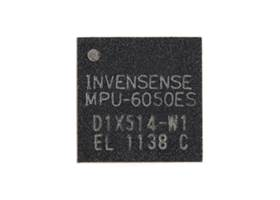
\includegraphics[width=0.5\textwidth]{figuras/mpu6050-sensor-top-straight.jpg}
    \fonte{o autor}
\end{figure}
A orientação dos sensores em relação ao encapsulamento obedece a regra da mão direita, conforme descrito na Figura~\ref{fig:mpu6050-diagram-axis}:
\begin{figure}[H]
    \centering
    \caption{Sensor MPU-6050 eixos em relação ao encapsulamento}\label{fig:mpu6050-diagram-axis}
    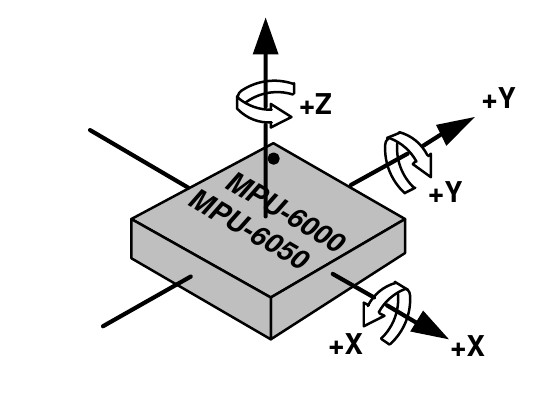
\includegraphics[width=0.5\textwidth]{figuras/mpu6050-diagram-axis.jpg}
    \fonte{\citeonline{mpu6050ps}}
\end{figure}
\begin{figure}[H]
    \centering
    \caption{Sensor MPU-6050 montado em placa módulo}\label{fig:mpu6050-board-top}
    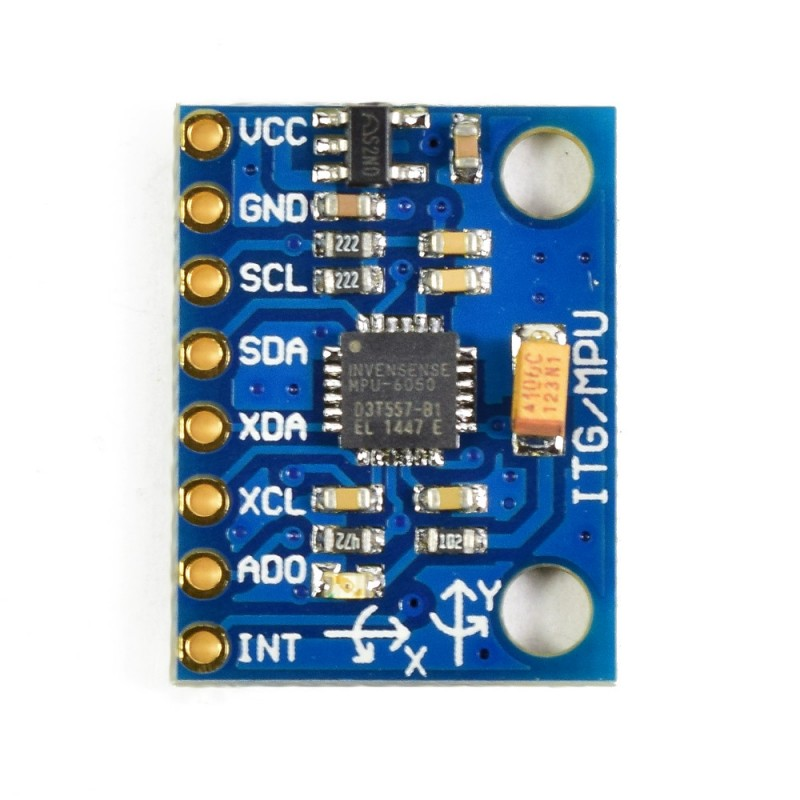
\includegraphics[width=0.5\textwidth]{figuras/mpu6050-board-top.jpg}
    \fonte{o autor}
\end{figure}
\begin{figure}[H]
    \centering
    \caption{Sensor MPU-6050 anexado à Raspberry Pi}\label{fig:mpu6050-proto-top}
    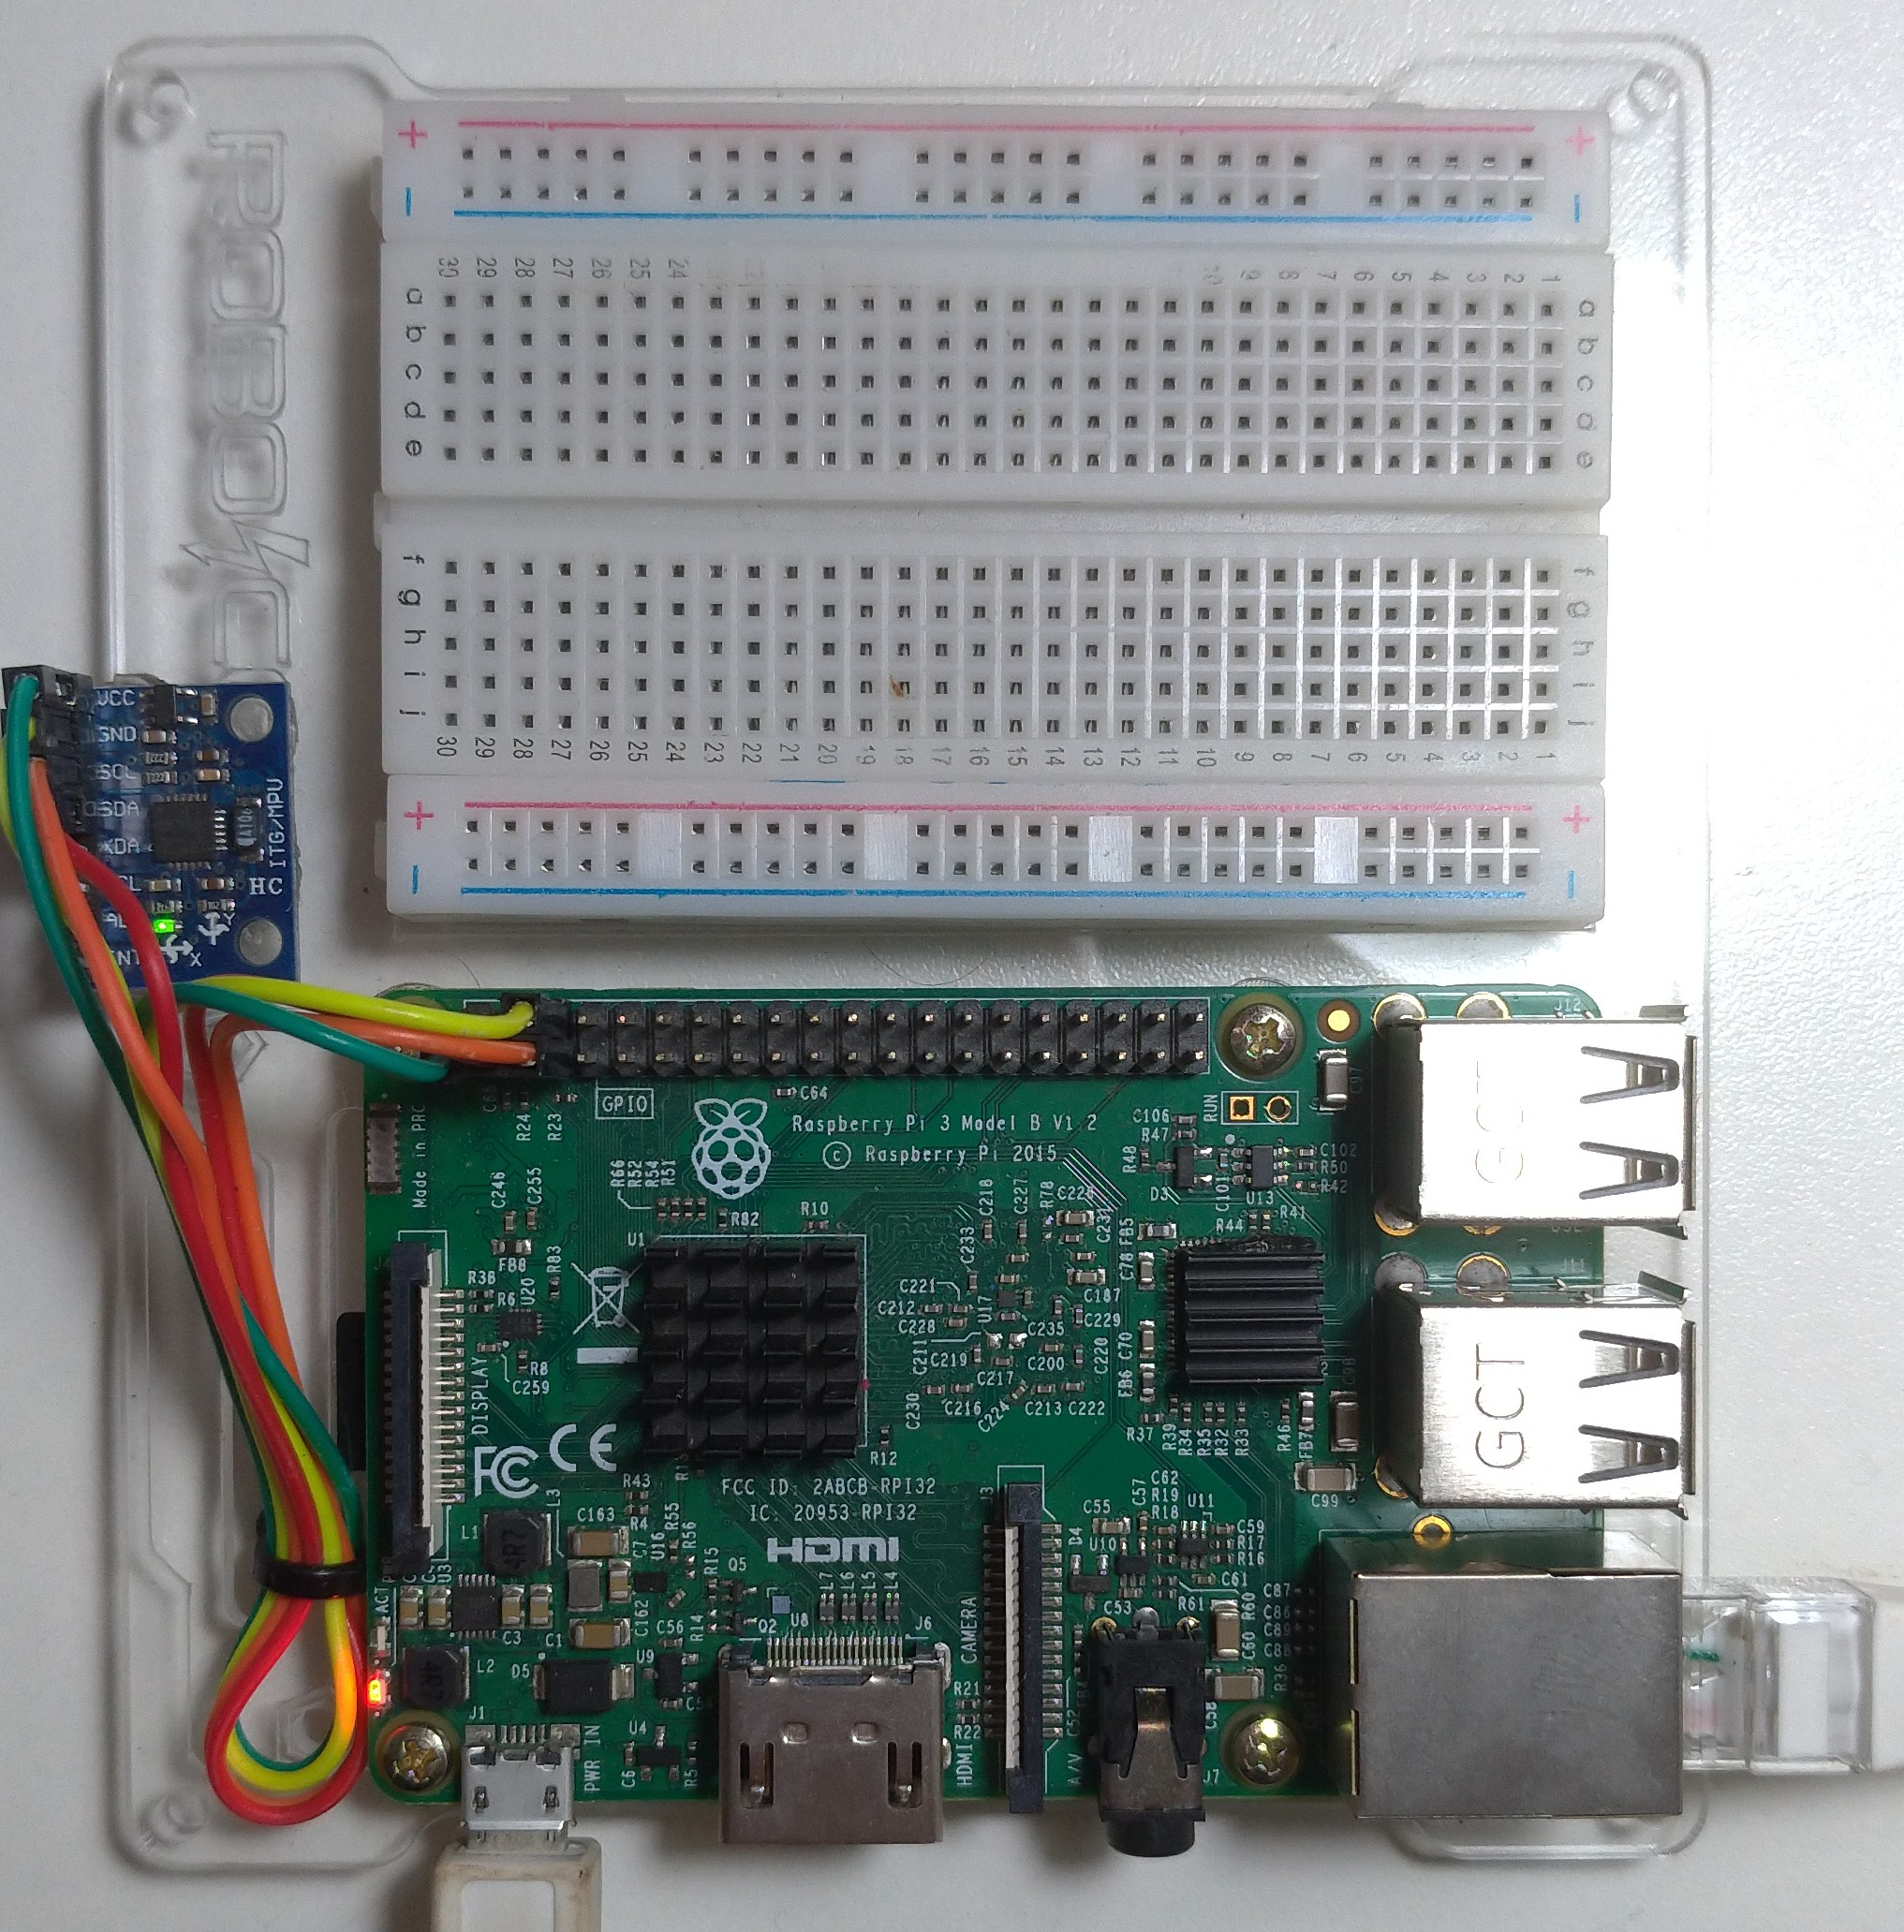
\includegraphics[width=0.5\textwidth]{figuras/mpu6050-proto-top.jpg}
    \fonte{o autor}
\end{figure}

Para a programação Utilizamos programação linguagem C para sistema Linux, com metologia ágil e desenvolvimento em código aberto.

\section{seleção de literatura com abordagens viáveis}

Após revisão abrangente, nos deparamos com métodos e abordagens bastante diversos para descrever a orientação de objetos e seus movimentos. Selecionamos as abordagens mais intuitivas e simples, que atendem ao objetivo de testar a viabilidade da aplicação desejada para os sensores.

\section{Elaboração de requisitos de software}

Após escolha da literatura aplicável, pudemos estabelecer os requisitos do software para obtenção de dados úteis dos sensores e os cuidados necessários.

\section{Desenvolvimento de software}

\section{ Testes de bancada para coleta de dados}

\section{ Análise dos dados}
